\documentclass[10pt]{article}
\usepackage[margin=0.6in]{geometry}
\usepackage{float}
\usepackage[T1]{fontenc}
\usepackage{lmodern}
\usepackage{amsmath}
\usepackage{graphicx}
\usepackage{booktabs}
\usepackage{caption}
\captionsetup{font=small,labelfont=bf,skip=3pt}
\setlength{\textfloatsep}{6pt}\setlength{\intextsep}{6pt}
\setlength{\parskip}{3pt}
\usepackage{microtype}
\pagestyle{empty}
\begin{document}
\begin{center}
{\large\bfseries Measuring Clutch Performance in Soccer When the Result Is on the Line}
\end{center}
\vspace{-6pt}
\noindent\textbf{Introduction}\\
Some moments in soccer matter far more than others: an equaliser in stoppage time, or a last-ditch block that protects a one-goal lead. Players who deliver in these moments are called clutch, yet clutch performance is hard to measure. Current approaches treat the final minutes as pressure or ask only what a goal for the team would change, overlooking that the next goal can go either way. We ask which players add the most value when the result is at stake, whether attacking or defending.

\noindent\textbf{Methods}\\
We use the public Wyscout event dataset (Pappalardo et al., 2019): 2.83 million actions from Europe's five top leagues in 2017/18. The pipeline has two branches (Figure~\ref{fig:pipeline}). Two gradient-boosted classifiers (CatBoost), validated on held-out leagues, measure how each action changes its team's chances of scoring and conceding. A logistic outcome model turns score, time left and home advantage into expected league points, giving every moment a gain if the team scores next ($L^{+}$) and a cost if it concedes next ($L^{-}$). Each action's clutch value weights its scoring change by $L^{+}$ and its conceding change by $L^{-}$; the Clutch Performance Index (CPI) averages this per 56 actions over a season, with intervals from resampling matches.

\noindent\textbf{Results}\\
The value of the next goal depends sharply on the score: late in a level game, scoring is worth 1.6 league points, but for a team one goal up, conceding costs 1.6 while scoring adds only 0.2. These stakes match real final results and track the true cost of conceding far better than a scoring-only measure (correlation 0.98 versus 0.39). CPI therefore rewards forwards who score when goals are needed and defenders and goalkeepers who protect leads; goal-saving actions earn 2.6 to 3 times more credit. Icardi, Bernardeschi, Laguardia and Oblak lead their positions (Table~\ref{tab:leaders}), and season CPI is stable (split-half reliability 0.51).

\noindent\textbf{Conclusion}\\
CPI gives clubs, analysts and broadcasters a measure of who delivered when results were decided, crediting attacking and defending on one scale for recruitment and match analysis.

\begin{figure}[H]
\centering
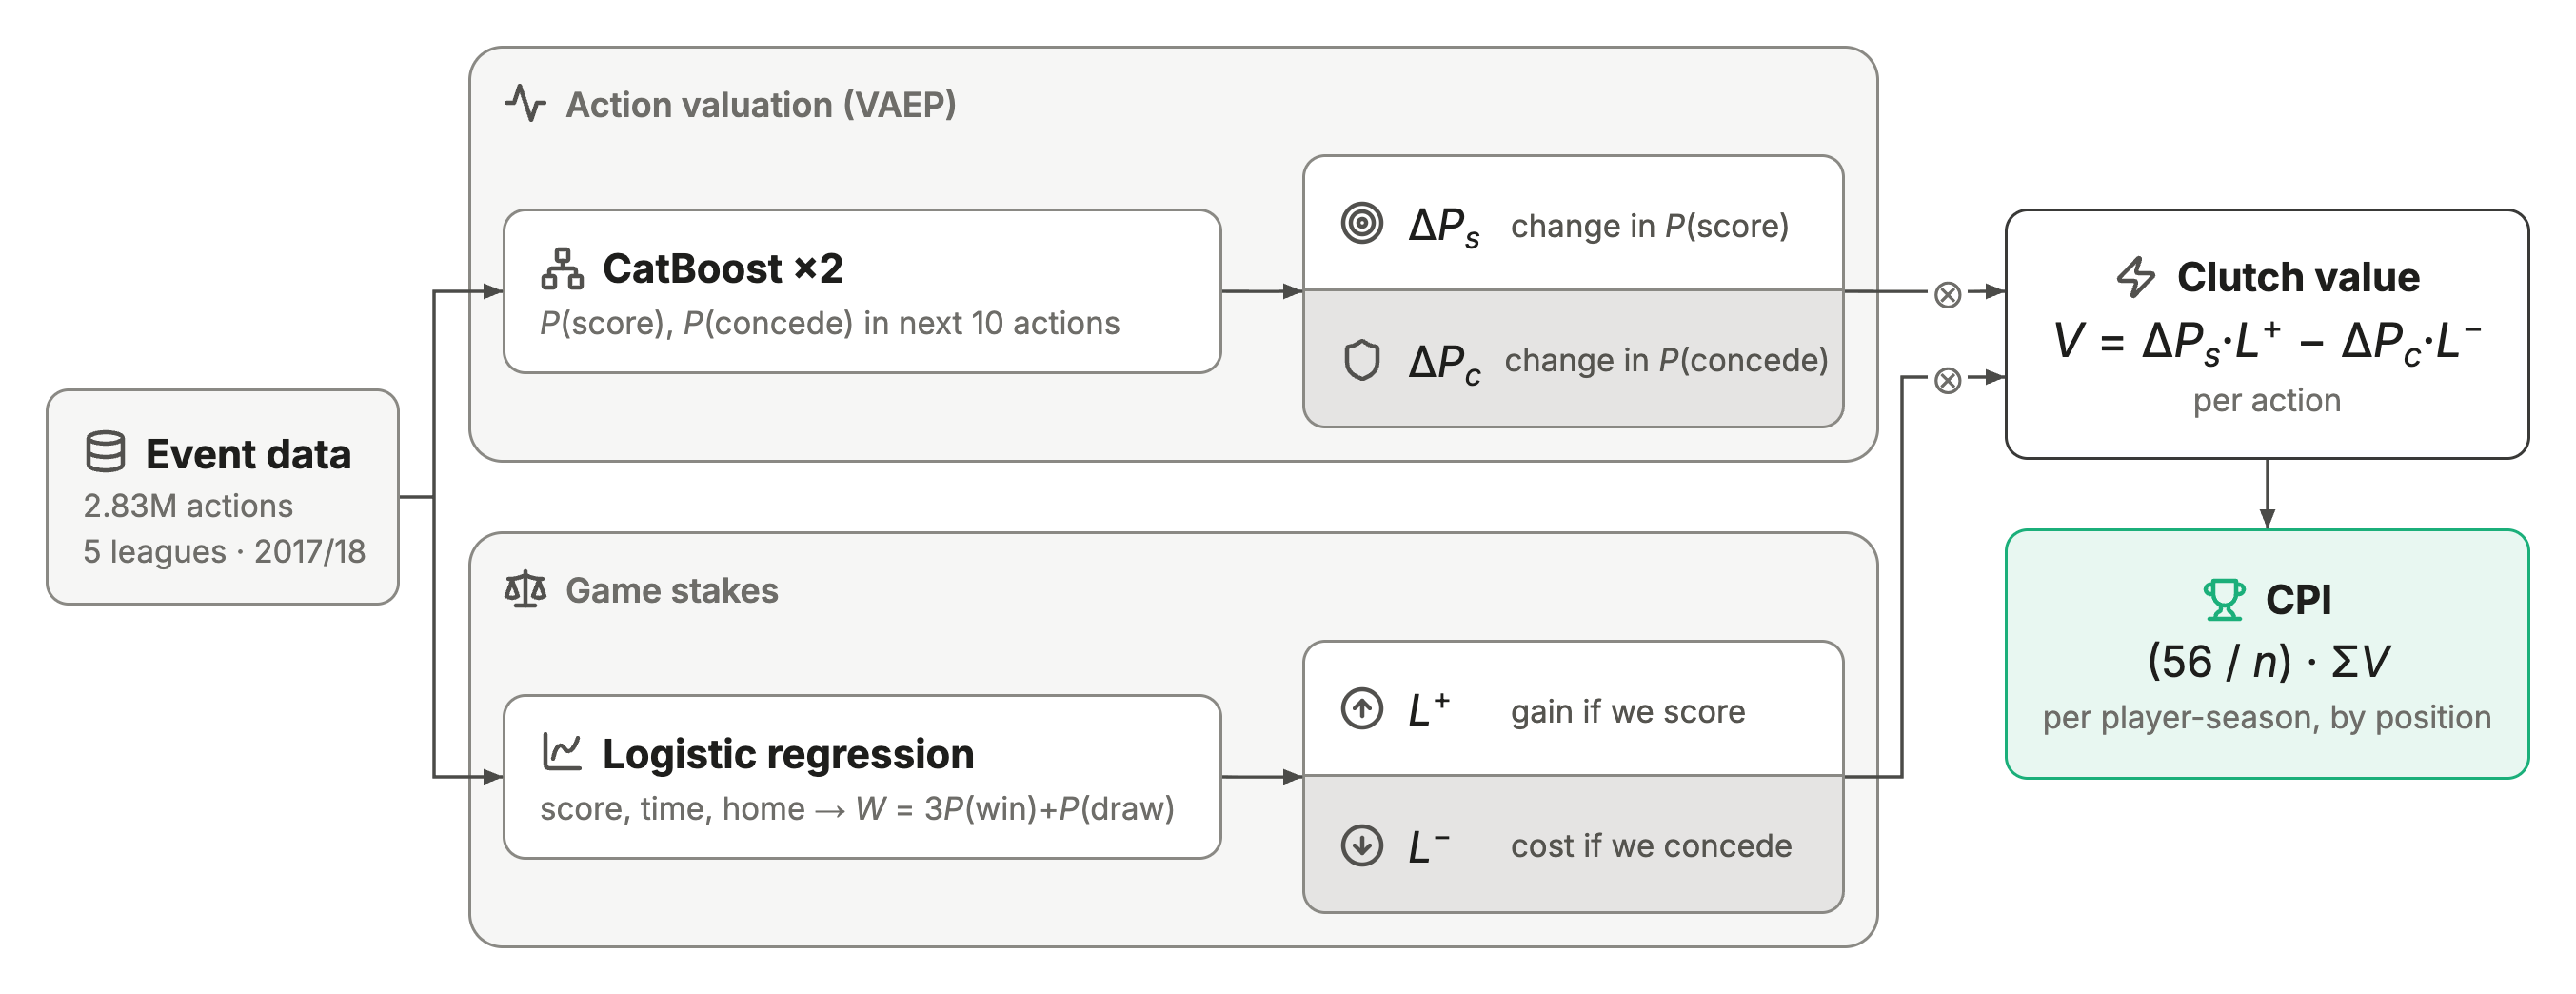
\includegraphics[width=0.82\linewidth]{pipeline_figure.png}
\vspace{-4pt}
\caption{Action values (top) weighted by the next goal's worth (bottom) give each action's clutch value and each player's CPI.}
\label{fig:pipeline}
\end{figure}

\begin{table}[H]
\centering
\footnotesize
\setlength{\tabcolsep}{6pt}
\renewcommand{\arraystretch}{0.95}
\caption{Top three per position: CPI (95\% CI), share of resamples in the top 10, and rank by plain action value; goalkeepers ranked on goal prevention.}
\label{tab:leaders}
\begin{tabular}{@{}l l c c c@{}}
\toprule
Position & Player & CPI (95\% CI) & Top-10 share & Plain rank \\
\midrule
Forwards & Icardi & 0.62 (0.22--1.06) & 83\% & 2 \\
 & Cavani & 0.50 (0.26--0.72) & 75\% & 1 \\
 & Immobile & 0.43 (0.16--0.71) & 53\% & 3 \\
\midrule
Midfielders & Bernardeschi & 0.32 (0.11--0.55) & 52\% & 17 \\
 & Kwon Chang-Hoon & 0.31 (0.13--0.53) & 56\% & 7 \\
 & Rony Lopes & 0.30 (0.15--0.46) & 47\% & 2 \\
\midrule
Defenders & Laguardia & 0.30 (0.09--0.56) & 74\% & 10 \\
 & Debuchy & 0.25 (0.10--0.42) & 68\% & 4 \\
 & Ramis & 0.22 (0.08--0.44) & 50\% & 6 \\
\midrule
Goalkeepers & Oblak & 0.28 (0.22--0.35) & 97\% & 38 \\
 & Oier & 0.24 (0.18--0.29) & 62\% & 11 \\
 & Guaita & 0.24 (0.19--0.29) & 66\% & 5 \\
\bottomrule
\end{tabular}
\end{table}
\end{document}
